\documentclass[conference]{IEEEtran}
\usepackage[spanish,es-nodecimaldot]{babel}
\usepackage{graphicx}
\usepackage{booktabs}
\usepackage{amsmath}
\usepackage{tikz}
\usetikzlibrary{arrows.meta,positioning,fit,backgrounds}
\usepackage{url}

\newcommand{\code}[1]{\texttt{\small #1}}
\emergencystretch=2em
\tolerance=2000
\hbadness=1500

\title{TrainingLab: planificaci\'on determinista, registro en el gimnasio y decisi\'on local asistida por un modelo de lenguaje peque\~no}

\author{
\IEEEauthorblockN{Alejandro Buend\'ia}
\IEEEauthorblockA{Proyecto Fitness --- BodyLab \& TrainingLab\\
Repositorio: \url{https://github.com/SCP-00/Fitness}\\
Proyecto personal de c\'odigo abierto}
}

\begin{document}
\maketitle

\begin{abstract}
TrainingLab es la mitad activa del ecosistema Fitness: la aplicaci\'on que
reparte el volumen de la semana, prescribe la sesi\'on del d\'ia seg\'un el
tiempo disponible, el estado de recuperaci\'on y el equipamiento real del
usuario, y registra las series con el m\'inimo n\'umero de gestos posible. Este
documento describe su dise\~no completo: la metodolog\'ia con la que se
estudiaron aplicaciones comerciales de referencia y se decidi\'o qu\'e adoptar
y qu\'e rechazar; la arquitectura de la aplicaci\'on; los motores
deterministas de sesi\'on y semana; el modelo local de decisi\'on y el asistente
basado en un modelo de lenguaje peque\~no que se ejecuta en el mismo equipo; cada
una de las interfaces --- incluida la pantalla inmersiva de entrenamiento --- con
su contrato de dise\~no; el flujo de producci\'on de material gr\'afico con su
postura de licencias; y el estado al que el proyecto quiere llegar.
El principio que ordena todas las decisiones es que \emph{el modelo propone y la
matem\'atica dispone}: ninguna sugerencia, humana o artificial, llega a la
pantalla sin validarse contra el equipamiento, las familias musculares y el
presupuesto de tiempo.
\end{abstract}

\begin{IEEEkeywords}
entrenamiento de fuerza, planificaci\'on de volumen, aplicaci\'on
\emph{local-first}, modelos de decisi\'on, modelos de lenguaje locales,
interfaz de usuario para m\'ovil.
\end{IEEEkeywords}

\section{Introducci\'on}

\subsection{Problema}
Las aplicaciones de registro de entrenamiento resuelven bien anotar series, pero
mal decidir. Las que proponen planes lo hacen desde un servidor, con un modelo
opaco que no explica su decisi\'on, sin conocer el equipamiento real del usuario
y sin respetar su presupuesto de tiempo. Adem\'as, la mayor\'ia convierte el
entrenamiento en una m\'etrica social: rachas que castigan, comparaciones
p\'ublicas y contenido que se descarga sin que el usuario lo haya pedido.

\subsection{Enfoque}
TrainingLab propone tres niveles expl\'icitos de inteligencia, en orden de
fiabilidad descendente:

\begin{enumerate}
  \item un \textbf{motor determinista} (\code{session.ts}, \code{week.ts},
  \code{validator.ts}) que no necesita inteligencia artificial alguna y que
  constituye el suelo del sistema;
  \item un \textbf{modelo local de decisi\'on} del tipo de decisi\'on tipada
  contextual, entrenado con el propio historial del usuario, con pesos acotados
  y explicaciones legibles;
  \item un \textbf{modelo de lenguaje local opcional} que se ejecuta sobre la
  interfaz de \emph{loopback}, con llamada a herramientas restringida por
  gram\'atica y con validaci\'on obligatoria de su propuesta final.
\end{enumerate}

\subsection{Aportaciones}
(1) La metodolog\'ia de dise\~no basada en el estudio de aplicaciones
comerciales, con el registro de lo adoptado y lo rechazado; (2) los motores de
planificaci\'on y su contrato de honestidad; (3) la arquitectura del asistente
local y su verificaci\'on medida; (4) la descripci\'on de cada interfaz,
incluida la pantalla inmersiva de entrenamiento; (5) el pipeline de material
gr\'afico con postura de licencias; y (6) la hoja de ruta por fases.

\section{Metodolog\'ia de dise\~no}

\subsection{Estudio de referencia}
Se estudiaron doce capturas de una aplicaci\'on comercial de referencia para
extraer \emph{patrones de interacci\'on} --- no arte, no iconos, no textos, no
marca. La distinci\'on es deliberada: los patrones de interacci\'on no son
expresi\'on protegible; los activos gr\'aficos s\'i, y por eso el material de
estudio vive en una carpeta ignorada por el sistema de control de versiones y
nunca se redistribuye. La Tabla~\ref{tab:patterns} resume el resultado.

\begin{table}[t]
\caption{Patrones estudiados: adoptado o rechazado}
\label{tab:patterns}
\centering
\footnotesize
\begin{tabular}{@{}p{40mm}p{9mm}p{27mm}@{}}
\toprule
Patr\'on & Adop. & C\'omo lo hacemos nosotros \\
\midrule
Tarjeta principal del entreno del d\'ia con una acci\'on & s\'i & hero con tiempo, familias y un \'unico bot\'on de inicio \\
Barra inferior de cinco destinos con acci\'on central & s\'i & Hoy, Ejercicios, Iniciar, Progreso, Ajustes \\
Buscador de ejercicios con hojas de filtro & s\'i & filtros por m\'usculo, equipo y categor\'ia \\
Ficha de ejercicio por pesta\~nas & s\'i & gu\'ia, resumen, rango, historial \\
Registro con tabla de series y columna ``anterior'' & s\'i & n\'ucleo de la pantalla inmersiva \\
Panel de progreso con m\'etrica, periodo y mapa de constancia & s\'i & todo calculado en local \\
``Eres el 27\,\% m\'as fuerte'' por percentiles & \textbf{no} & no tenemos datos poblacionales: nivel estimado propio, etiquetado como referencia interna \\
\emph{Feed} social y seguidores & \textbf{no} & contradice el modelo de privacidad \\
Racha como presi\'on psicol\'ogica & parcial & constancia sin lenguaje de castigo \\
\bottomrule
\end{tabular}
\end{table}

\subsection{Principios de dise\~no}
Siete reglas resuelven las discusiones durante la implementaci\'on: una pantalla,
un trabajo; el pulgar manda en la mitad inferior; medir, no decorar; el modelo
propone y la matem\'atica dispone; \emph{sin conexi\'on no es un modo}, es el
estado normal; texto de interfaz en espa\~nol e identificadores en ingl\'es; y
la paleta naranja brasa sobre negro casi puro no cambia sin el consentimiento del
autor.

\section{Arquitectura}

TrainingLab es una aplicaci\'on independiente que comparte el cat\'alogo de
ejercicios con BodyLab a trav\'es del alias del monorepositorio, de manera que
funciona sola --- con su propio diccionario de idioma, su propia base de datos y
su propia interfaz --- sin duplicar ni un dato del cat\'alogo. La persistencia es
IndexedDB por dispositivo; el historial compartido del hogar es una opci\'on
expl\'icita con interruptor visible en la cabecera de preferencias y nunca se
activa sola. El empaquetado de escritorio usa Tauri~2 y la l\'ogica permanece
sin dependencias de plataforma.

Dos decisiones de datos merecen menci\'on. Primero, la \textbf{unidad can\'onica
es el kilogramo} en almacenamiento, historial compartido y exportaci\'on; la
libra es una preferencia de presentaci\'on, con la constante exacta
$1\,\text{kg} = 2{,}2046226218488\,\text{lb}$ mostrada en la propia interfaz
para que la conversi\'on sea auditable. Segundo, cada grupo de ajustes tiene
valores por defecto a prueba de migraci\'on, de modo que un registro antiguo se
completa con los valores nuevos sin romper la lectura.

\section{Motores deterministas}

\subsection{Sesi\'on del d\'ia}
\code{session.ts} construye la sesi\'on a partir de cinco entradas: presupuesto
de tiempo, estado de recuperaci\'on (energ\'ia, motivaci\'on y frescura, cada uno
de 1 a 5), equipamiento disponible, familias musculares con debilidad declarada
o medida, y la asignaci\'on semanal. La funci\'on \emph{nunca lanza una
excepci\'on}: ante entradas degeneradas degrada y explica. Su comportamiento
medido: con energ\'ia m\'axima produce 22 series y 57 minutos; con energ\'ia baja
produce 18 series, 46 minutos y un RIR m\'as alto --- es decir, \emph{m\'as
reserva cuando el usuario est\'a fatigado}; y sin equipamiento se queda en peso
corporal con un aviso expl\'icito. La opci\'on \code{focusFamilies}, a\~nadida
para el planificador semanal, es aditiva y compatible hacia atr\'as: filtra por
familia de la ranura sin tocar recuperaci\'on, equipamiento ni techo de volumen.

\subsection{Semana}
\code{week.ts} reparte familias musculares entre los d\'ias de entrenamiento con
cuatro reglas duras: \textbf{recuperaci\'on de 48 horas} (ninguna familia grande
en dos d\'ias de entrenamiento consecutivos), \textbf{d\'ebil primero},
\textbf{frecuencia doble} para el tercio m\'as d\'ebil cuando hay al menos tres
d\'ias, y \textbf{presupuesto por d\'ia}. Lo que no cabe no se oculta: queda
listado como no cubierto con su motivo. La distribuci\'on de d\'ias usa una
funci\'on determinista (\code{spreadTrainingDays}), y el n\'umero de d\'ias
semanales (2 a 6) es una preferencia del usuario que regenera el reparto. Nueve
pruebas fijan estas promesas, incluida la de no lanzar con entradas
degeneradas: cero d\'ias, cat\'alogo vac\'io y todas las familias bloqueadas.

\subsection{Calentamiento}
El generador de calentamiento implementa la petici\'on m\'as votada durante
a\~nos en los foros de las comunidades de referencia, y lo hace con tres
propiedades que la comunidad espera: una rampa de porcentajes hacia la primera
serie de trabajo (barra vac\'ia, 50\,\%, 70\,\% y 85\,\% con 8, 5, 3 y 1
repeticiones), series \textbf{fuera del volumen} --- nunca cuentan para el d\'ia,
la semana ni un r\'ecord --- y \textbf{descanso propio}, deliberadamente m\'as
corto. Cuando el ejercicio no tiene carga externa, la rampa se sustituye por una
l\'inea de movilidad en lugar de inventar porcentajes; durante el desarrollo se
detect\'o y corrigi\'o un defecto real en ese caso, que imprim\'ia un valor nulo
en pantalla.

\subsection{R\'ecords y esfuerzo}
\code{records.ts} contiene la l\'ogica pura de r\'ecords y de finalizaci\'on de
prescripci\'on, con la estimaci\'on de una repetici\'on m\'axima por la
f\'ormula de Epley
\begin{equation}
\hat{e}1RM = w \left(1 + \frac{r}{30}\right),
\end{equation}
redondeada exactamente igual que en BodyLab para que las dos aplicaciones nunca
discrepen sobre el mismo conjunto de datos. El esfuerzo se registra por serie en
RIR, que es la variable que el planificador usa despu\'es para ajustar volumen.

\section{Modelo local de decisi\'on}
El segundo nivel es un modelo de decisi\'on del tipo de decisi\'on tipada
contextual --- la clase comercial a la que pertenecen los modelos que eligen una
acci\'on discreta con explicaci\'on, no los modelos generativos de texto ---
implementado como un \emph{bandido} contextual con las siguientes propiedades:
un prior determinista, actualizaciones en l\'inea a partir de los resultados
registrados por el usuario, pesos acotados para que una racha no desestabilice
el sistema, una funci\'on de explicaci\'on legible y una se\~nal de deriva. Se
persiste como JSON y no sale del equipo. Es importante ser precisos en la
descripci\'on: es un modelo local \emph{de esa clase}, y ni es ni pretende ser
el producto comercial de terceros del que tomamos la idea, ni un modelo
predictivo del mundo (JEPA). Esta distinci\'on se mantiene tambi\'en en la
documentaci\'on del repositorio.

\section{Asistente con modelo de lenguaje local}

\subsection{Alcance}
El tercer nivel es opcional y apagado por defecto. Habla la interfaz de
\emph{API} de estilo abierto sobre \emph{loopback}, de modo que funciona con los
servidores locales habituales sin acoplarse a ninguno, y no requiere conexi\'on.
El modelo recibe herramientas y las usa para explorar antes de proponer; la
propuesta final es una llamada a una herramienta terminal
(\code{propose\_session} para el d\'ia y \code{propose\_week} para la semana)
que el sistema \emph{valida antes de mostrar}: identificadores existentes en el
cat\'alogo, equipamiento disponible, familias coherentes con la asignaci\'on y
ajuste al presupuesto de tiempo. Si la validaci\'on falla, la propuesta no llega
a la pantalla.

\subsection{Restricci\'on por gram\'atica}
La literatura y la pr\'actica coinciden en que los modelos peque\~nos s\'olo
hacen llamada a herramientas de forma fiable cuando la salida se restringe. Por
eso el asistente se apoya en decodificaci\'on restringida por gram\'atica, una
por tarea y con decodificaci\'on voraz, y en que el servidor genere la
gram\'atica a partir del esquema de las herramientas. El bucle de herramientas
est\'a acotado: el modelo explora y termina, o el sistema corta.

\subsection{Verificaci\'on medida}
La prueba no es una descripci\'on sino una ejecuci\'on real con un modelo de 4
mil millones de par\'ametros en el equipo del autor: ante la instrucci\'on
``energ\'ia 2 sobre 5, enfoca isquiotibiales y gl\'uteos'', el modelo explor\'o el
cat\'alogo con cuatro llamadas de herramienta y cerr\'o con una propuesta a los
81 segundos; redujo el volumen de empuje y tracci\'on de cinco a tres series,
subi\'o la reserva y priorizó el grupo m\'as d\'ebil, y \textbf{todos los
identificadores propuestos exist\'ian en el cat\'alogo}. La conclusi\'on honesta:
para un modelo de ese tama\~no el resultado es s\'olido pero lento, y es
exactamente el comportamiento dise\~nado --- el modelo propone, la matem\'atica
dispone.

\subsection{Paquete de conocimiento}
El asistente se acompa\~na de un paquete de conocimiento \emph{generado} a partir
del cat\'alogo (143 ejercicios, sus rasgos y su material) y de la descripci\'on
de las herramientas, con una prueba de \emph{no deriva}: si alguien modifica el
cat\'alogo y no regenera el paquete, la prueba falla. El paquete incluye la
gu\'ia de ejecuci\'on para los servidores locales m\'as usados y la receta de
gram\'aticas por tarea.

\section{Interfaces}

\subsection{Modelo de navegaci\'on}
La versi\'on actual concentra todo en una p\'agina de 1559 l\'ineas con dos
paneles tras un interruptor. El dise\~no objetivo son \textbf{cinco destinos
reales} con sincronizaci\'on por \emph{hash} (\code{\#/hoy},
\code{\#/ejercicios}, \code{\#/progreso}, \code{\#/ajustes}), que aporta tres
cosas: el gesto de retroceso del tel\'efono funciona, los enlaces profundos a la
ficha de un ejercicio son triviales y las pruebas de navegador pueden direccionar
una pantalla directamente. En tel\'efono la navegaci\'on es una barra inferior
con acci\'on central; en escritorio, un ra\'il lateral con densidad de teclado.
La Tabla~\ref{tab:tl-screens} describe cada destino.

\begin{table}[t]
\caption{Destinos y pantallas de TrainingLab}
\label{tab:tl-screens}
\centering
\footnotesize
\begin{tabular}{@{}p{19mm}p{57mm}@{}}
\toprule
Destino & Contenido y acci\'on principal \\
\midrule
Hoy & hero de la sesi\'on, estado de recuperaci\'on, lista de ranuras, semana plegada; ``empezar'' \\
Ejercicios & buscador, filtros por m\'usculo, equipo y categor\'ia, recientes; ``a\~nadir a la sesi\'on'' \\
Iniciar & arranque directo de la sesi\'on, sesi\'on libre y generaci\'on con el asistente \\
Progreso & m\'etrica y periodo, cifra principal con variaci\'on, gr\'afico, indicadores, constancia, r\'ecords \\
Ajustes & equipo, preferencias del plan, coach local, datos de BodyLab, historial del hogar \\
\bottomrule
\end{tabular}
\end{table}

\subsection{Hoy}
Es la \'unica pantalla que puede estar por encima del pliegue. La tarjeta
principal muestra el tiempo presupuestado, las familias del d\'ia, el n\'umero de
ejercicios y una miniatura muscular, con un \'unico bot\'on de inicio; debajo, el
estado de recuperaci\'on en tres controles compactos que \emph{recalculan el plan
en el sitio} con una l\'inea que explica qu\'e cambi\'o; la lista de ranuras con
series, repeticiones, carga, sustituci\'on y gu\'ia; y la semana plegada. El
estado vac\'io no culpa a la red: ofrece importar el archivo de BodyLab o usar el
cat\'alogo interno (que es tambi\'en el camino del invitado en la red local). La
Fig.~\ref{fig:tl-today} muestra el estado actual en escritorio.

\begin{figure}[t]
\centering
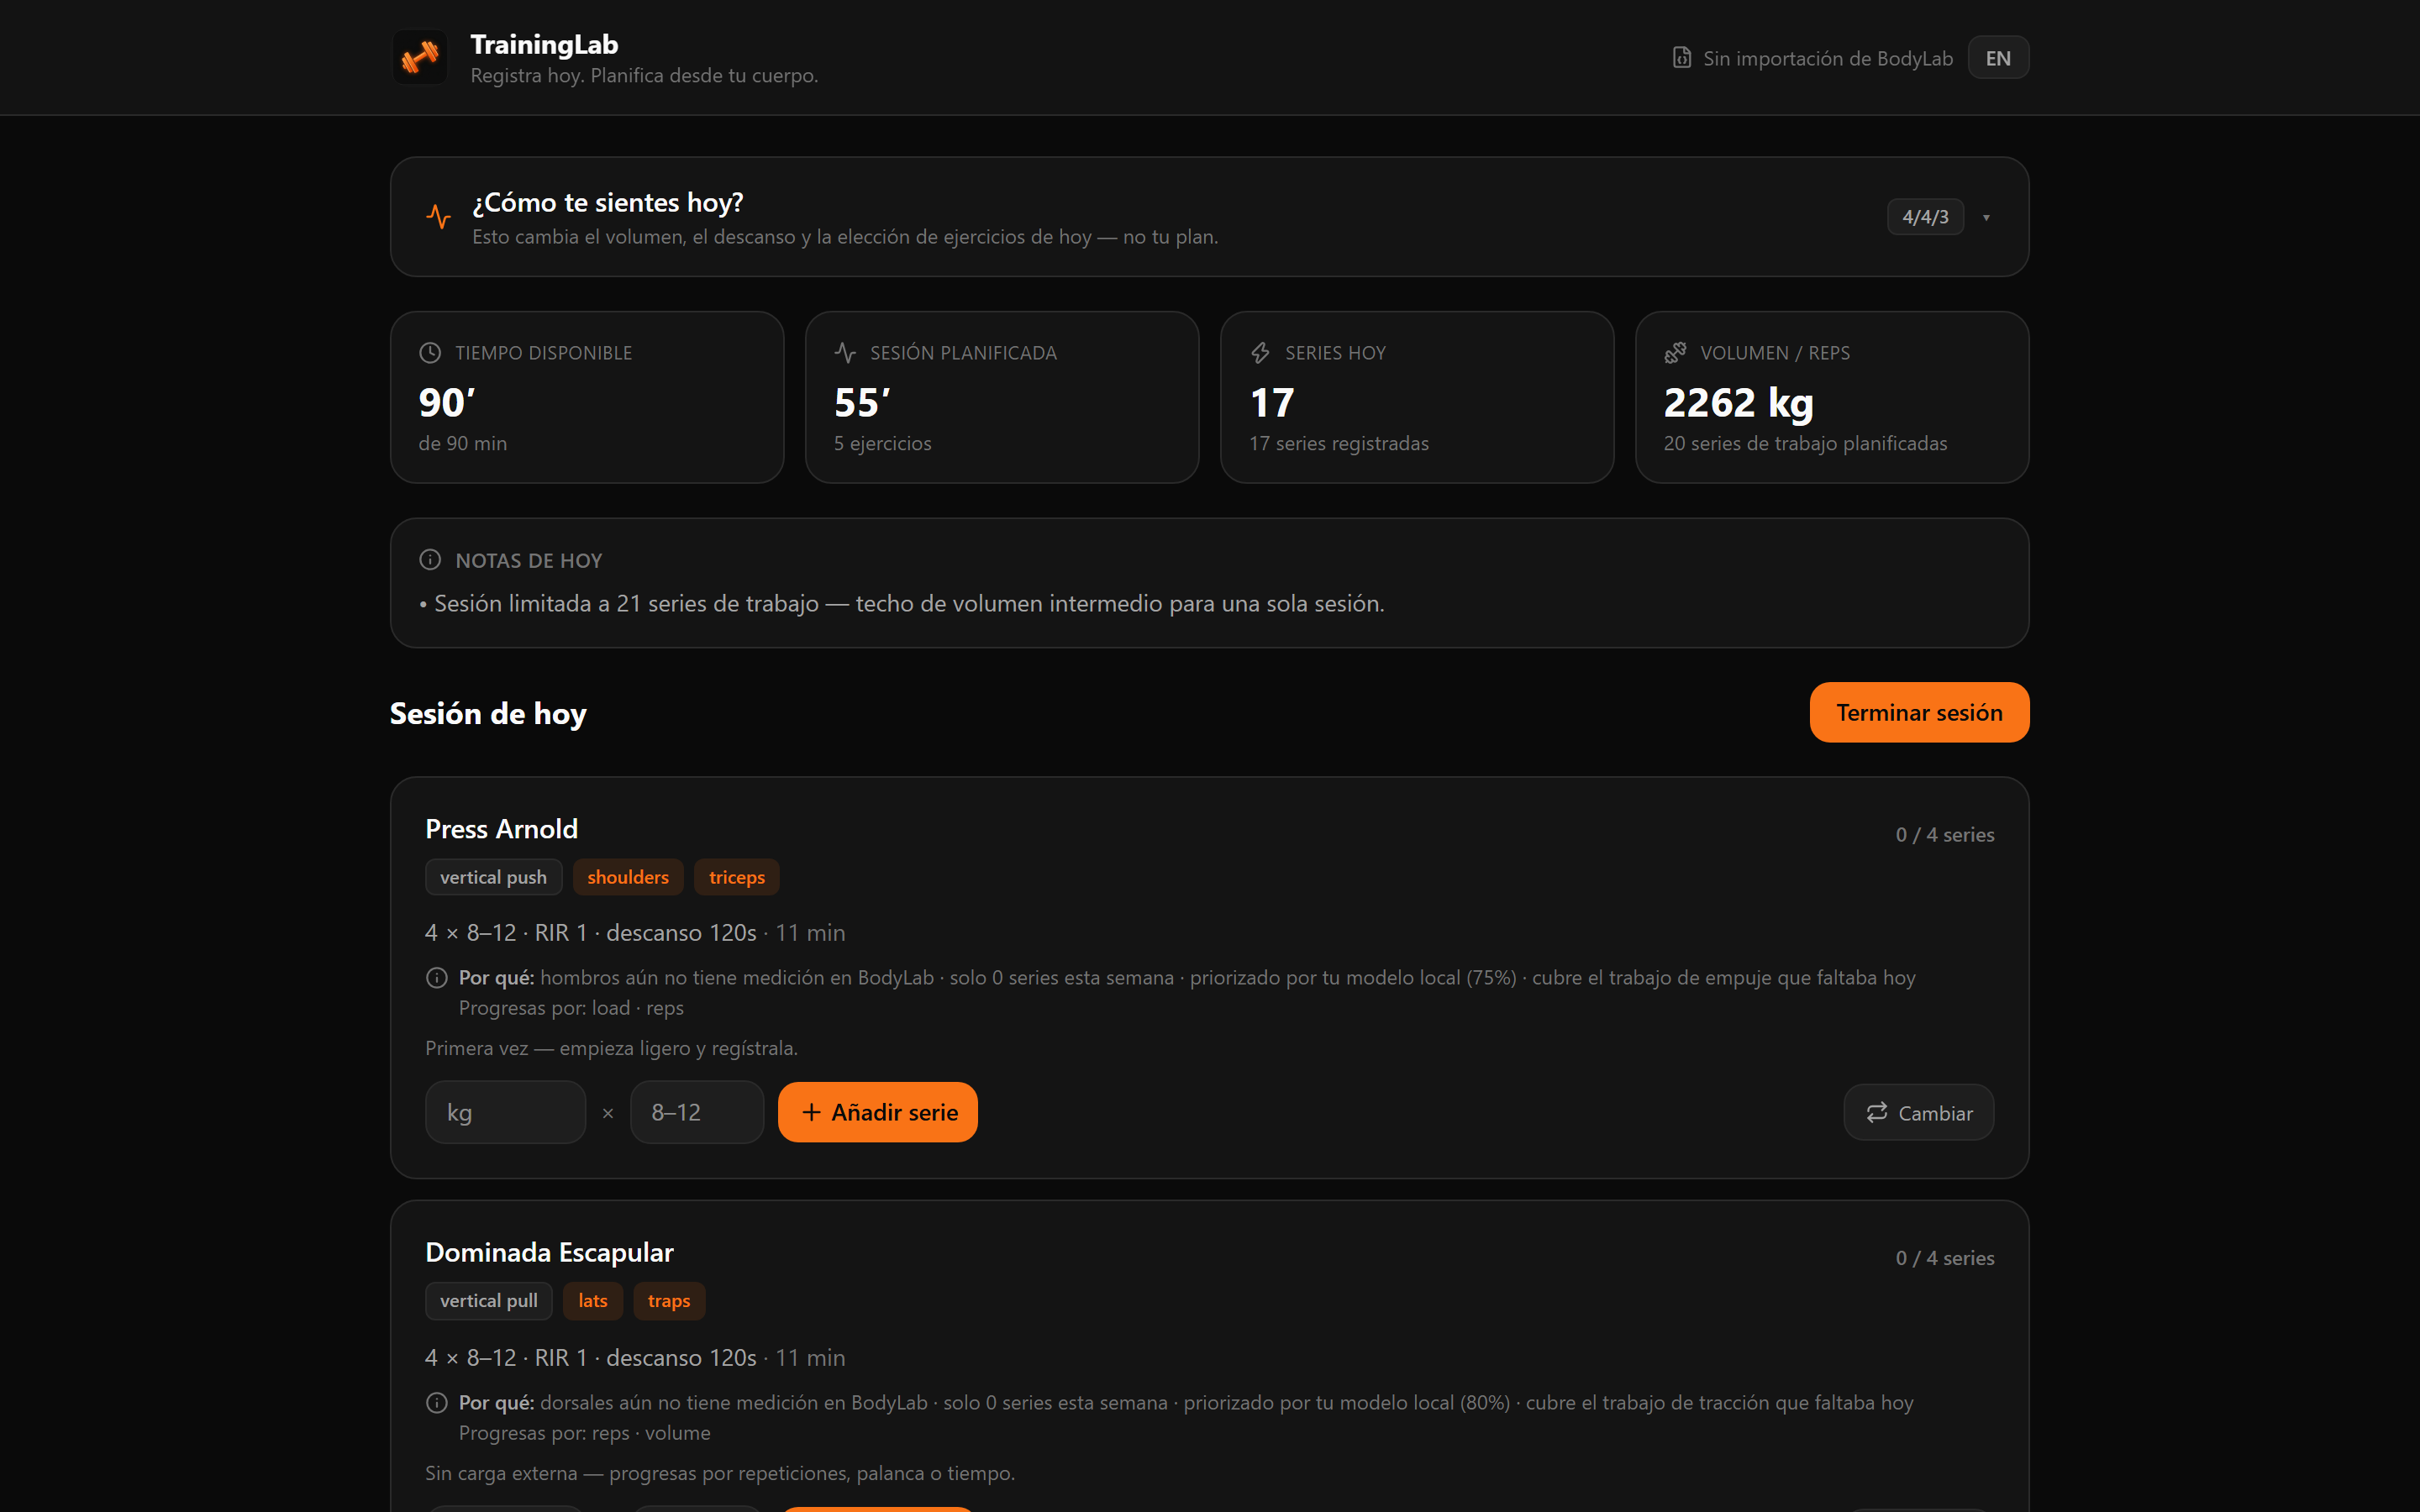
\includegraphics[width=\columnwidth]{../screenshots/traininglab-today.png}
\caption{Pantalla Hoy: estado de recuperaci\'on, sesi\'on planificada con
justificaci\'on por ejercicio y reparto semanal.}
\label{fig:tl-today}
\end{figure}

\subsection{Sesi\'on inmersiva (ZEN)}
La pantalla de entrenamiento es la pieza con m\'as valor de uso: reduce la
interfaz a lo que se necesita entre series. El dise\~no objetivo a\~nade tres
elementos que hoy no existen y que son los de mayor rendimiento por l\'inea de
c\'odigo:

\begin{itemize}
  \item una \textbf{columna ``anterior''} en la tabla de series, que muestra lo
  que se hizo la \'ultima vez en esa misma serie;
  \item \textbf{marcas de tipo de serie} --- calentamiento, \emph{dropset} y
  fallo --- con color, haciendo visible que el calentamiento no cuenta para el
  volumen;
  \item el \textbf{esfuerzo por serie} como control principal, con el texto
  escrito adem\'as del n\'umero (``quedan 2 repeticiones en reserva''), y una
  barra de descanso pegada al borde inferior, propiedad del servicio de
  cron\'ometro y no de un di\'alogo.
\end{itemize}

La Fig.~\ref{fig:zen} es el esquema de esa pantalla. El cierre de sesi\'on
conserva el banner y el sonido de celebraci\'on, que son visuales y
sintetizados, no ficheros de audio con licencia.

\begin{figure}[t]
\centering
\begin{tikzpicture}[font=\scriptsize, x=1mm, y=1mm]
\draw[rounded corners=2pt, thick] (0,0) rectangle (84,62);
\draw[fill=black!6] (0,54) rectangle (84,62);
\draw[thick] (3,57.5) -- (5.5,60) -- (8,57.5);
\node[anchor=west] at (10,58) {12:41};
\node[anchor=east] at (81,58) {$\cdots$};
\node[draw, fill=black!10, minimum width=34mm, minimum height=20mm] at (42,40) {\textbf{imagen / dibujo del ejercicio}};
\node[anchor=west] at (3,32) {\textbf{Press de banca con barra}};
\node[anchor=west] at (3,27) {Pectoral mayor $\cdot$ Tr\'iceps $\cdot$ Hombro anterior};
\node[draw, rounded corners=1pt] at (14,21) {Gu\'ia};
\node[draw, rounded corners=1pt] at (30,21) {Sustituir};
\node[draw, rounded corners=1pt] at (46,21) {Notas};
\node[anchor=west] at (3,15) {\textbf{SERIE}\quad \textbf{ANTERIOR}\quad \textbf{KG}\quad \textbf{REPS}};
\node[anchor=west] at (3,10) {\; 1\quad\quad 60$\times$8\quad\quad [ 60 ]\quad [ 8 ]};
\node[anchor=west] at (3,5.5) {\; 2\quad\quad 60$\times$8\quad\quad [ 60 ]\quad [ 8 ]};
\node[anchor=west] at (3,1) {\; C\quad\quad ---\quad\quad\;\, [ 40 ]\quad [ 10 ]\;\; calentamiento};
\draw[fill=black!6] (0,-8) rectangle (84,0);
\node[anchor=west] at (4,-4) {Esfuerzo de la serie (RIR) [1][2][3][4][5]};
\draw[fill=black!12] (0,-16) rectangle (84,-8);
\node[anchor=west] at (4,-12) {Descanso 1:30 \quad iniciar \quad saltar};
\end{tikzpicture}
\caption{Esquema de la pantalla inmersiva: media, nombre y familias,
acciones de gu\'ia y sustituci\'on, tabla de series con columna anterior y tipo
de serie, esfuerzo por serie y barra de descanso fija.}
\label{fig:zen}
\end{figure}

\subsection{Ejercicios y ficha}
La biblioteca usa el cat\'alogo compartido: buscador insensible a acentos en los
dos idiomas, filtros por m\'usculo, equipo y categor\'ia en hojas inferiores, y
filas que muestran miniatura, subt\'itulo muscular, equipo, dificultad y si
existe gu\'ia. La ficha se organiza en cuatro pesta\~nas: \emph{gu\'ia}
(instrucciones numeradas, errores frecuentes, seguridad y respiraci\'on),
\emph{resumen} (m\'usculos con foco primario o secundario y equipo),
\emph{rango} (evoluci\'on del propio rendimiento estimado) e \emph{historial}
(todas las series registradas, agrupadas por fecha). A\~nadir a la sesi\'on es
una acci\'on de primera clase en cada fila cuando hay sesi\'on abierta, que es lo
que hace r\'apida la sustituci\'on desde la pantalla inmersiva.

\subsection{Progreso}
Selectores de m\'etrica (volumen, series, repeticiones, tiempo) y de periodo
(semana, mes, trimestre, a\~no); cifra principal con variaci\'on y el rango de
fechas exacto, nunca un incremento sin ancla; un gr\'afico de tendencia
implementado en el propio c\'odigo, sin dependencia de terceros y con alternativa
accesible en tabla; indicadores de entrenamientos, r\'ecords y d\'ias; un mapa de
constancia tipo calendario con vocabulario neutro --- constancia, no castigo ---;
y el \textbf{equilibrio muscular} por familia frente a una banda de referencia,
calculado con las mismas familias que usa el planificador, de modo que la
pantalla no puede contradecir al plan. El ``nivel estimado'' por familia se
publica con sus umbrales visibles y etiquetado como referencia interna.

\subsection{Semana y ajustes}
La tarjeta semanal muestra una l\'inea por d\'ia de entrenamiento con sus
familias, el d\'ia de hoy marcado, y permite regenerar. Los ajustes agrupan en un
\'unico men\'u plegable el asistente local, los datos de BodyLab, el historial
compartido y el acceso m\'ovil, con el interruptor de red visible en la cabecera
para encender y apagar la red del hogar en un solo gesto; el equipamiento y las
preferencias del plan quedan fuera de ese men\'u porque se usan a diario.

\subsection{Contrato de interfaz}
La Tabla~\ref{tab:tl-contract} recoge las reglas verificadas en dispositivo
real, todas obligatorias (Fig.~\ref{fig:tl-phone}).

\begin{table}[t]
\caption{Contrato de interfaz de TrainingLab}
\label{tab:tl-contract}
\centering
\footnotesize
\begin{tabular}{@{}p{21mm}p{51mm}@{}}
\toprule
Regla & Compromiso \\
\midrule
Cortes de dise\~no & una columna bajo 640\,px; columna centrada hasta 1023; todos los paneles a la vez desde 1024 \\
Objetivos t\'actiles & $\geq 44$\,px en tel\'efono, incluidas las cabeceras plegables \\
Campos de entrada & $\geq 16$\,px de tipograf\'ia (evita el zoom autom\'atico) \\
Zonas seguras & \code{viewport-fit=cover} y \code{env(safe-area-inset-*)}; barra inferior con margen propio \\
Altura & \code{100dvh}; sin rebote horizontal \\
Hojas modales & Inferior con esquinas superiores redondeadas y desplazamiento interno \\
Idioma & Diccionario \'unico espa\~nol/ingl\'es, sin literales en el marcado \\
\bottomrule
\end{tabular}
\end{table}

\begin{figure}[t]
\centering
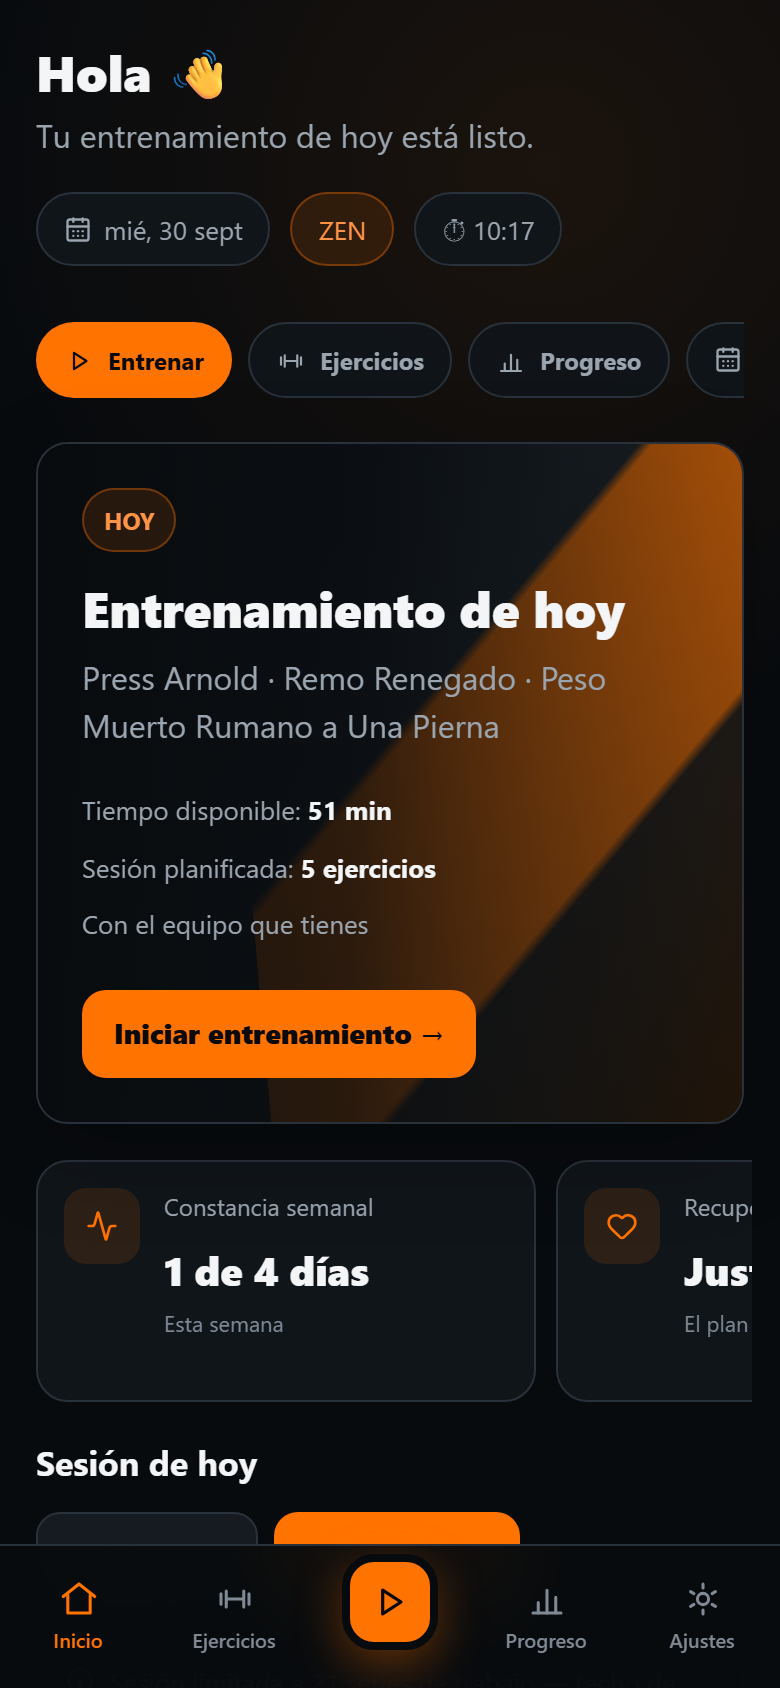
\includegraphics[width=0.70\columnwidth]{../screenshots/traininglab-phone.png}
\caption{Vista de tel\'efono con la barra de navegaci\'on inferior y el contrato
de objetivos t\'actiles.}
\label{fig:tl-phone}
\end{figure}

\subsection{C\'omo se presentan ejercicios y planes}\label{sec:plans}
Cinco reglas de presentaci\'on, que son la respuesta al requisito de c\'omo
mostrar el contenido en un entorno local:
\begin{enumerate}
  \item un plan se muestra siempre \textbf{como semana y como d\'ia}, nunca como
  un formulario;
  \item cada serie planificada lleva su \textbf{evidencia} a un toque: por qu\'e
  ese ejercicio, por qu\'e ese n\'umero de series, por qu\'e esa carga;
  \item \textbf{editar es de primera clase} (sustituir, a\~nadir, quitar,
  reordenar, reajustar el tiempo) y la edici\'on manual se recuerda;
  \item el \textbf{calentamiento se ve pero no pesa}: aparece en la sesi\'on,
  queda fuera de la aritm\'etica del volumen y est\'a etiquetado;
  \item \textbf{ning\'un estado vac\'io es un callej\'on}: siempre hay una
  acci\'on siguiente.
\end{enumerate}

\section{Pipeline de material gr\'afico}

\subsection{Cascada y licencias}
La presentaci\'on de un movimiento usa una cascada que nunca deja un hueco:
animaci\'on licenciada, par de fotograf\'ias de dominio p\'ublico, y dibujo
propio animado por el \emph{rig} de movimiento como \'ultimo recurso. De 143
ejercicios, 100 tienen material real (36 animaciones y 64 pares de fotos) y 43
caen al dibujo propio; las bibliotecas con licencia que proh\'ibe la
redistribuci\'on se descartaron de forma expl\'icita.

\subsection{Siluetas generadas localmente}
Para cerrar esas 43 entradas sin usar material ajeno se construy\'o un pipeline
de generaci\'on local con tres decisiones de dise\~no:

\textbf{La entrada no es una imagen ajena, es nuestro propio esqueleto.} Someter
las capturas de otra aplicaci\'on a un proceso de imagen a imagen producir\'ia
una obra derivada de su arte. En su lugar, el \emph{rig} que ya codifica los 28
patrones renderiza mapas de postura en el formato can\'onico de puntos
anatom\'icos que los modelos de control saben leer: 28 im\'agenes para los 143
ejercicios, todas nuestras, con la biomec\'anica correcta porque la escribimos
nosotros. El modelo aporta el aspecto; la verdad mec\'anica la aporta el motor.

\textbf{El hardware acota el modelo.} En el equipo del autor (6\,GB de memoria de
v\'ideo) se define un nivel ligero verificado de 5{,}3\,GB (modelo base y red de
control) con 3--8 segundos por imagen, y un nivel de calidad con destilaci\'on de
cuatro pasos que requiere gesti\'on de memoria y tarda 15--45 segundos. Los
modelos de mayor tama\~no se descartan por no caber.

\textbf{La salida se revisa antes de publicarse.} La generaci\'on escribe en un
directorio de preparaci\'on y s\'olo un comando expl\'icito copia el material a
las dos aplicaciones y lo registra en el manifiesto, sin sustituir nunca a un
recurso existente y anotando su origen. La semilla es determinista en funci\'on
del identificador del ejercicio, de modo que una repetici\'on reproduce la misma
imagen; y los ejercicios cardiovasculares se excluyen por defecto, porque en
ellos una silueta no ense\~na nada que un tiempo no enseñe mejor.

\section{Calidad y operaciones}
La puerta de verificaci\'on local se ejecuta completa antes de publicar:
\textbf{815 pruebas de n\'ucleo} en 49 archivos, \textbf{110 pruebas de interfaz},
\textbf{21 flujos de extremo a extremo} en navegador real, an\'alisis est\'atico
sin avisos, tipos estrictos y compilaciones de producci\'on de las dos
aplicaciones. La integraci\'on continua vive en la ra\'iz del repositorio, y la
publicaci\'on construye ambos instaladores, publica un alias estable para que los
enlaces de descarga sobrevivan a las versiones, y firma \'unicamente cuando los
secretos existen. La actualizaci\'on de escritorio es manual y opcional: se
consulta cuando el usuario lo pide. La demostraci\'on p\'ublica de las dos
aplicaciones se despliega en cada publicaci\'on.

\section{Estado actual y hoja de ruta}
Ya funcionan: el motor de sesi\'on con recuperaci\'on y equipamiento, el
planificador semanal con la regla de 48 horas, el generador de calentamiento, la
preferencia de kilogramos o libras con su constante exacta, la pantalla inmersiva
en su primera versi\'on, la tarjeta semanal, el paquete de conocimiento del
asistente y el pipeline de material. La Tabla~\ref{tab:roadmap} ordena lo que
falta, con el esfuerzo estimado.

\begin{table}[t]
\caption{Hoja de ruta de interface}
\label{tab:roadmap}
\centering
\footnotesize
\begin{tabular}{@{}p{8mm}p{48mm}p{14mm}@{}}
\toprule
Fase & Alcance & Esfuerzo \\
\midrule
P0 & armaz\'on: separar la p\'agina \'unica en pantallas con navegaci\'on y sincronizaci\'on por \emph{hash} & M \\
P1 & biblioteca y ficha de ejercicio con sus cuatro pesta\~nas & L \\
P2 & pantalla inmersiva completa: columna anterior, tipos de serie, esfuerzo por serie, barra de descanso & M \\
P3 & progreso: selectores, gr\'afico, indicadores, mapa de constancia, equilibrio muscular & L \\
P4 & edici\'on de la semana y hoja de propuesta del asistente con su rastro de razones & M \\
\bottomrule
\end{tabular}
\end{table}

El objetivo declarado para el conjunto es que medir, entrenar y volver a medir
sean un solo ciclo: la debilidad medida en BodyLab alimenta el plan, el plan se
registra en TrainingLab y el resultado vuelve como dato. Nada de ese ciclo
necesita un servidor, y ninguna propuesta --- ni del modelo local ni del modelo
de lenguaje --- llega a la pantalla sin pasar por las reglas duras.

\section{Conclusiones}
TrainingLab demuestra que una aplicaci\'on de entrenamiento puede ser
inteligente sin ser opaca: la inteligencia se organiza en tres niveles, el
primero de ellos sin inteligencia artificial, y los otros dos con la misma
disciplina de validaci\'on. La interfaz se dise\~n\'o a partir de patrones de
interacci\'on estudiados en el mercado pero con decisiones expl\'icitas de
rechazo en lo que contradice la privacidad o la honestidad de los n\'umeros. El
trabajo pendiente es de organizaci\'on de la interfaz --- cinco pantallas en
lugar de una --- y de contenido: cerrar la biblioteca con material propio
generado localmente y completar la pantalla inmersiva.

\begin{thebibliography}{9}
\bibitem{plan} Proyecto Fitness. \emph{Plan de dise\~no de interfaz de
TrainingLab}. Documento de dise\~no del repositorio, 2026.
\bibitem{uicontract} Proyecto Fitness. \emph{Contrato de dise\~no de interfaz y
reglas responsivas}. Documento de dise\~no del repositorio, 2026.
\bibitem{research} Proyecto Fitness. \emph{Validaci\'on de caracter\'isticas:
investigaci\'on de comunidades china y estadounidense}. Documento de
investigaci\'on del repositorio, 2026.
\bibitem{audit} Proyecto Fitness. \emph{Auditor\'ia de datos de ejercicios y
cobertura del cat\'alogo}. Documento de auditor\'ia del repositorio, 2026.
\bibitem{epley} B.~Epley, \emph{Poundage Chart}, 1985 (estimaci\'on de una
repetici\'on m\'axima).
\bibitem{gbnf} Documentaci\'on de decodificaci\'on restringida por gram\'atica
de los servidores locales de modelos de lenguaje, 2026.
\end{thebibliography}

\end{document}
